\documentclass{standalone}
\usepackage{tikz}
\usetikzlibrary{patterns, positioning}
\usepackage[sfdefault]{ClearSans} %% option 'sfdefault' activates Clear Sans as the default text font
\usepackage[T1]{fontenc}

\begin{document}
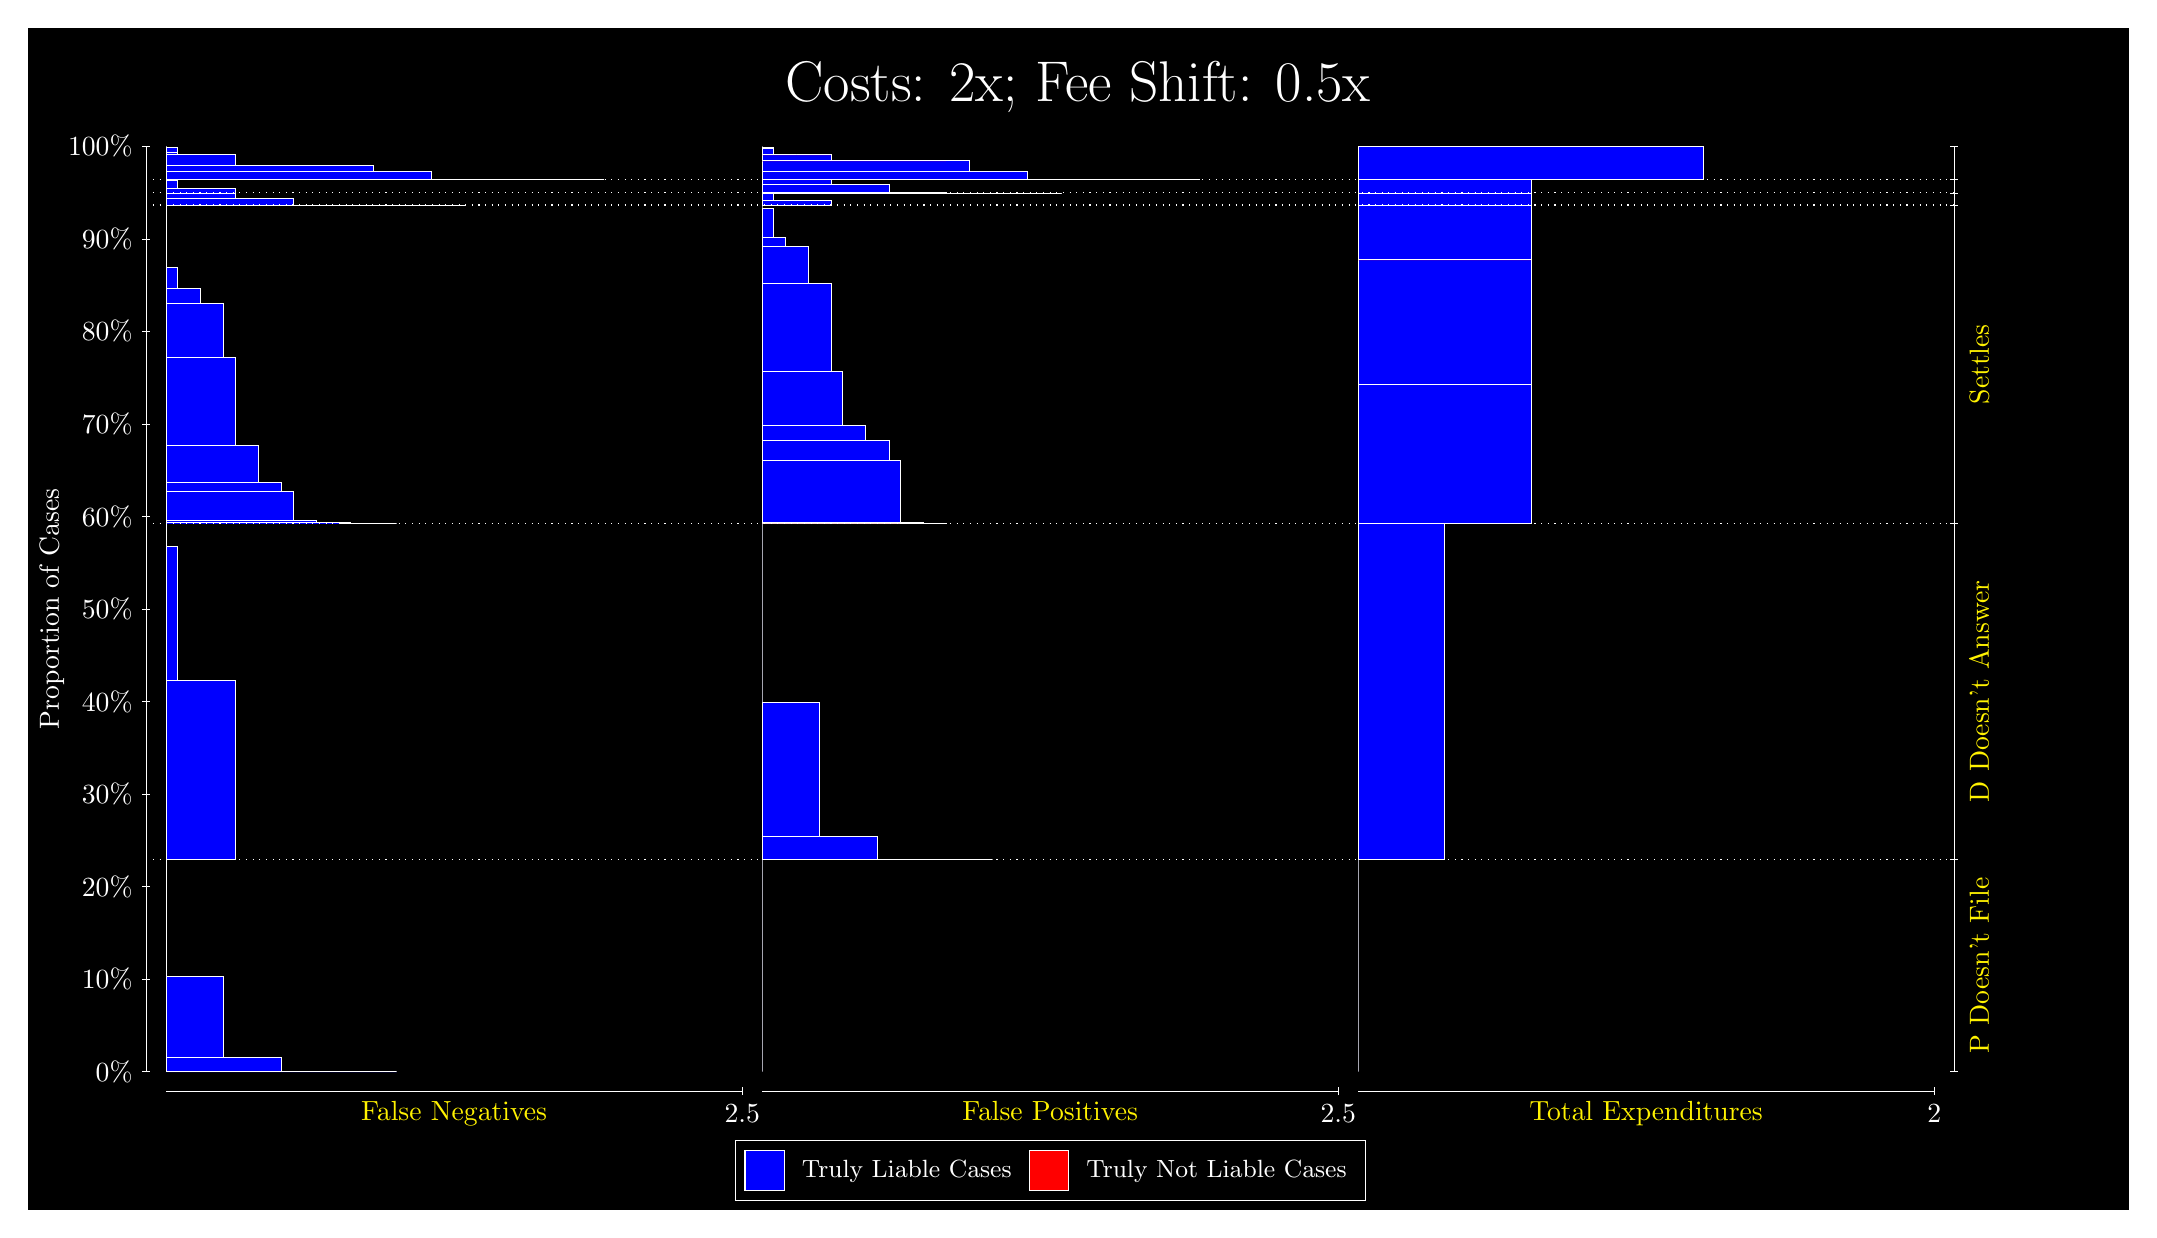
\begin{tikzpicture}
\draw[fill=black] (0,0) rectangle (26.667,15);
\draw[text=white] (0,13.5) rectangle (26.667,15) node[midway] {\huge Costs: 2x; Fee Shift: 0.5x};
\draw[white, very thin] (1.5,1.75) -- (1.5,13.5);
\node[rotate=90, text=white, anchor=center] at (0.3, 7.625) {Proportion of Cases};
\draw[white, very thin] (1.45,1.75) -- (1.55,1.75);
\node[text=white, anchor=east] at (1.45, 1.75) {0\%};
\draw[white, very thin] (1.45,2.925) -- (1.55,2.925);
\node[text=white, anchor=east] at (1.45, 2.925) {10\%};
\draw[white, very thin] (1.45,4.1) -- (1.55,4.1);
\node[text=white, anchor=east] at (1.45, 4.1) {20\%};
\draw[white, very thin] (1.45,5.275) -- (1.55,5.275);
\node[text=white, anchor=east] at (1.45, 5.275) {30\%};
\draw[white, very thin] (1.45,6.45) -- (1.55,6.45);
\node[text=white, anchor=east] at (1.45, 6.45) {40\%};
\draw[white, very thin] (1.45,7.625) -- (1.55,7.625);
\node[text=white, anchor=east] at (1.45, 7.625) {50\%};
\draw[white, very thin] (1.45,8.8) -- (1.55,8.8);
\node[text=white, anchor=east] at (1.45, 8.8) {60\%};
\draw[white, very thin] (1.45,9.975) -- (1.55,9.975);
\node[text=white, anchor=east] at (1.45, 9.975) {70\%};
\draw[white, very thin] (1.45,11.15) -- (1.55,11.15);
\node[text=white, anchor=east] at (1.45, 11.15) {80\%};
\draw[white, very thin] (1.45,12.325) -- (1.55,12.325);
\node[text=white, anchor=east] at (1.45, 12.325) {90\%};
\draw[white, very thin] (1.45,13.5) -- (1.55,13.5);
\node[text=white, anchor=east] at (1.45, 13.5) {100\%};

\draw[white, very thin] (24.457,1.75) -- (24.457,13.5);
\draw[white, very thin] (24.407,1.75) -- (24.507,1.75);
\node[anchor=west] at (24.407, 1.75) {};
\draw[white, very thin] (24.407,4.4441) -- (24.507,4.4441);
\node[anchor=west] at (24.407, 4.4441) {};
\draw[white, very thin] (24.407,8.7102) -- (24.507,8.7102);
\node[anchor=west] at (24.407, 8.7102) {};
\draw[white, very thin] (24.407,12.755) -- (24.507,12.755);
\node[anchor=west] at (24.407, 12.755) {};
\draw[white, very thin] (24.407,12.909) -- (24.507,12.909);
\node[anchor=west] at (24.407, 12.909) {};
\draw[white, very thin] (24.407,13.079) -- (24.507,13.079);
\node[anchor=west] at (24.407, 13.079) {};
\draw[white, very thin] (24.407,13.5) -- (24.507,13.5);
\node[anchor=west] at (24.407, 13.5) {};

\draw[white, very thin, fill=blue] (1.75,1.75) rectangle (4.6775,1.75);
\draw[white, very thin, fill=blue] (1.75,1.75) rectangle (3.9457,1.7515);
\draw[white, very thin, fill=blue] (1.75,1.7515) rectangle (3.2138,1.9331);
\draw[white, very thin, fill=blue] (1.75,1.9331) rectangle (2.4819,2.9596);
\draw[white, very thin, fill=red] (1.75,2.9596) rectangle (1.75,2.9596);
\draw[white, very thin, fill=blue] (1.75,2.9596) rectangle (1.75,4.4441);
\draw[white, very thin, fill=blue] (1.75,4.4441) rectangle (2.6283,6.7163);
\draw[white, very thin, fill=blue] (1.75,6.7163) rectangle (1.8964,8.4217);
\draw[white, very thin, fill=red] (1.75,8.4217) rectangle (1.75,8.4217);
\draw[white, very thin, fill=blue] (1.75,8.4217) rectangle (1.75,8.7102);
\draw[white, very thin, fill=blue] (1.75,8.7102) rectangle (4.6775,8.7102);
\draw[white, very thin, fill=blue] (1.75,8.7102) rectangle (4.3848,8.7103);
\draw[white, very thin, fill=blue] (1.75,8.7103) rectangle (4.092,8.7205);
\draw[white, very thin, fill=blue] (1.75,8.7205) rectangle (3.9457,8.7209);
\draw[white, very thin, fill=blue] (1.75,8.7209) rectangle (3.6529,8.752);
\draw[white, very thin, fill=blue] (1.75,8.752) rectangle (3.3602,9.1251);
\draw[white, very thin, fill=blue] (1.75,9.1251) rectangle (3.2138,9.2365);
\draw[white, very thin, fill=blue] (1.75,9.2365) rectangle (2.921,9.7063);
\draw[white, very thin, fill=blue] (1.75,9.7063) rectangle (2.6283,10.821);
\draw[white, very thin, fill=blue] (1.75,10.821) rectangle (2.4819,11.504);
\draw[white, very thin, fill=blue] (1.75,11.504) rectangle (2.1891,11.693);
\draw[white, very thin, fill=blue] (1.75,11.693) rectangle (1.8964,11.958);
\draw[white, very thin, fill=red] (1.75,11.958) rectangle (1.75,11.958);
\draw[white, very thin, fill=blue] (1.75,11.958) rectangle (1.75,12.755);
\draw[white, very thin, fill=blue] (1.75,12.755) rectangle (5.5558,12.755);
\draw[white, very thin, fill=blue] (1.75,12.755) rectangle (4.8239,12.755);
\draw[white, very thin, fill=blue] (1.75,12.755) rectangle (4.092,12.757);
\draw[white, very thin, fill=blue] (1.75,12.757) rectangle (3.3602,12.843);
\draw[white, very thin, fill=blue] (1.75,12.843) rectangle (2.6283,12.909);
\draw[white, very thin, fill=red] (1.75,12.909) rectangle (1.75,12.909);
\draw[white, very thin, fill=blue] (1.75,12.909) rectangle (2.6283,12.973);
\draw[white, very thin, fill=blue] (1.75,12.973) rectangle (1.8964,13.074);
\draw[white, very thin, fill=red] (1.75,13.074) rectangle (1.75,13.074);
\draw[white, very thin, fill=blue] (1.75,13.074) rectangle (1.75,13.079);
\draw[white, very thin, fill=blue] (1.75,13.079) rectangle (7.3123,13.079);
\draw[white, very thin, fill=blue] (1.75,13.079) rectangle (6.5805,13.079);
\draw[white, very thin, fill=blue] (1.75,13.079) rectangle (5.8486,13.086);
\draw[white, very thin, fill=blue] (1.75,13.086) rectangle (5.1167,13.182);
\draw[white, very thin, fill=blue] (1.75,13.182) rectangle (4.8239,13.182);
\draw[white, very thin, fill=blue] (1.75,13.182) rectangle (4.3848,13.258);
\draw[white, very thin, fill=blue] (1.75,13.258) rectangle (4.092,13.258);
\draw[white, very thin, fill=blue] (1.75,13.258) rectangle (3.6529,13.258);
\draw[white, very thin, fill=blue] (1.75,13.258) rectangle (3.3602,13.26);
\draw[white, very thin, fill=blue] (1.75,13.26) rectangle (2.921,13.26);
\draw[white, very thin, fill=blue] (1.75,13.26) rectangle (2.6283,13.262);
\draw[white, very thin, fill=blue] (1.75,13.262) rectangle (2.6283,13.396);
\draw[white, very thin, fill=blue] (1.75,13.396) rectangle (1.8964,13.429);
\draw[white, very thin, fill=blue] (1.75,13.429) rectangle (1.8964,13.494);
\draw[white, very thin, fill=red] (1.75,13.494) rectangle (1.75,13.494);
\draw[white, very thin, fill=blue] (1.75,13.494) rectangle (1.75,13.5);
\draw[white, very thin, fill=red] (9.3189,1.75) rectangle (9.3189,1.75);
\draw[white, very thin, fill=blue] (9.3189,1.75) rectangle (9.3189,4.4441);
\draw[white, very thin, fill=red] (9.3189,4.4441) rectangle (12.246,4.4441);
\draw[white, very thin, fill=blue] (9.3189,4.4441) rectangle (12.246,4.4441);
\draw[white, very thin, fill=blue] (9.3189,4.4441) rectangle (11.515,4.4456);
\draw[white, very thin, fill=blue] (9.3189,4.4456) rectangle (10.783,4.7326);
\draw[white, very thin, fill=blue] (9.3189,4.7326) rectangle (10.051,6.438);
\draw[white, very thin, fill=blue] (9.3189,6.438) rectangle (9.3189,8.7102);
\draw[white, very thin, fill=red] (9.3189,8.7102) rectangle (11.661,8.7102);
\draw[white, very thin, fill=blue] (9.3189,8.7102) rectangle (11.661,8.7168);
\draw[white, very thin, fill=red] (9.3189,8.7168) rectangle (11.368,8.7168);
\draw[white, very thin, fill=blue] (9.3189,8.7168) rectangle (11.368,8.7219);
\draw[white, very thin, fill=red] (9.3189,8.7219) rectangle (11.075,8.7219);
\draw[white, very thin, fill=blue] (9.3189,8.7219) rectangle (11.075,9.5074);
\draw[white, very thin, fill=blue] (9.3189,9.5074) rectangle (10.929,9.7722);
\draw[white, very thin, fill=blue] (9.3189,9.7722) rectangle (10.636,9.9608);
\draw[white, very thin, fill=blue] (9.3189,9.9608) rectangle (10.344,10.644);
\draw[white, very thin, fill=blue] (9.3189,10.644) rectangle (10.197,11.759);
\draw[white, very thin, fill=blue] (9.3189,11.759) rectangle (9.9044,12.229);
\draw[white, very thin, fill=blue] (9.3189,12.229) rectangle (9.6116,12.34);
\draw[white, very thin, fill=blue] (9.3189,12.34) rectangle (9.4652,12.713);
\draw[white, very thin, fill=blue] (9.3189,12.713) rectangle (9.3189,12.755);
\draw[white, very thin, fill=red] (9.3189,12.755) rectangle (10.197,12.755);
\draw[white, very thin, fill=blue] (9.3189,12.755) rectangle (10.197,12.821);
\draw[white, very thin, fill=blue] (9.3189,12.821) rectangle (9.4652,12.907);
\draw[white, very thin, fill=blue] (9.3189,12.907) rectangle (9.3189,12.909);
\draw[white, very thin, fill=red] (9.3189,12.909) rectangle (13.125,12.909);
\draw[white, very thin, fill=blue] (9.3189,12.909) rectangle (13.125,12.909);
\draw[white, very thin, fill=blue] (9.3189,12.909) rectangle (12.393,12.909);
\draw[white, very thin, fill=blue] (9.3189,12.909) rectangle (11.661,12.914);
\draw[white, very thin, fill=blue] (9.3189,12.914) rectangle (10.929,13.014);
\draw[white, very thin, fill=blue] (9.3189,13.014) rectangle (10.197,13.079);
\draw[white, very thin, fill=red] (9.3189,13.079) rectangle (14.881,13.079);
\draw[white, very thin, fill=blue] (9.3189,13.079) rectangle (14.881,13.079);
\draw[white, very thin, fill=red] (9.3189,13.079) rectangle (14.149,13.079);
\draw[white, very thin, fill=blue] (9.3189,13.079) rectangle (14.149,13.079);
\draw[white, very thin, fill=red] (9.3189,13.079) rectangle (13.417,13.079);
\draw[white, very thin, fill=blue] (9.3189,13.079) rectangle (13.417,13.085);
\draw[white, very thin, fill=red] (9.3189,13.085) rectangle (12.686,13.085);
\draw[white, very thin, fill=blue] (9.3189,13.085) rectangle (12.686,13.182);
\draw[white, very thin, fill=blue] (9.3189,13.182) rectangle (11.954,13.318);
\draw[white, very thin, fill=red] (9.3189,13.318) rectangle (11.661,13.318);
\draw[white, very thin, fill=blue] (9.3189,13.318) rectangle (11.661,13.318);
\draw[white, very thin, fill=blue] (9.3189,13.318) rectangle (11.222,13.32);
\draw[white, very thin, fill=red] (9.3189,13.32) rectangle (10.929,13.32);
\draw[white, very thin, fill=blue] (9.3189,13.32) rectangle (10.929,13.32);
\draw[white, very thin, fill=blue] (9.3189,13.32) rectangle (10.49,13.32);
\draw[white, very thin, fill=blue] (9.3189,13.32) rectangle (10.197,13.395);
\draw[white, very thin, fill=red] (9.3189,13.395) rectangle (10.197,13.395);
\draw[white, very thin, fill=blue] (9.3189,13.395) rectangle (10.197,13.397);
\draw[white, very thin, fill=blue] (9.3189,13.397) rectangle (9.758,13.397);
\draw[white, very thin, fill=blue] (9.3189,13.397) rectangle (9.4652,13.469);
\draw[white, very thin, fill=blue] (9.3189,13.469) rectangle (9.4652,13.493);
\draw[white, very thin, fill=blue] (9.3189,13.493) rectangle (9.3189,13.5);
\draw[white, very thin, fill=red] (16.888,1.75) rectangle (16.888,1.75);
\draw[white, very thin, fill=blue] (16.888,1.75) rectangle (16.888,4.4441);
\draw[white, very thin, fill=red] (16.888,4.4441) rectangle (17.986,4.4441);
\draw[white, very thin, fill=blue] (16.888,4.4441) rectangle (17.986,8.7102);
\draw[white, very thin, fill=red] (16.888,8.7102) rectangle (19.083,8.7102);
\draw[white, very thin, fill=blue] (16.888,8.7102) rectangle (19.083,10.479);
\draw[white, very thin, fill=red] (16.888,10.479) rectangle (19.083,10.479);
\draw[white, very thin, fill=blue] (16.888,10.479) rectangle (19.083,12.06);
\draw[white, very thin, fill=red] (16.888,12.06) rectangle (19.083,12.06);
\draw[white, very thin, fill=blue] (16.888,12.06) rectangle (19.083,12.755);
\draw[white, very thin, fill=red] (16.888,12.755) rectangle (19.083,12.755);
\draw[white, very thin, fill=blue] (16.888,12.755) rectangle (19.083,12.909);
\draw[white, very thin, fill=red] (16.888,12.909) rectangle (19.083,12.909);
\draw[white, very thin, fill=blue] (16.888,12.909) rectangle (19.083,13.079);
\draw[white, very thin, fill=red] (16.888,13.079) rectangle (21.279,13.079);
\draw[white, very thin, fill=blue] (16.888,13.079) rectangle (21.279,13.5);
\draw[white, dotted] (1.5,4.4441) -- (24.457,4.4441);
\draw[white, dotted] (1.5,8.7102) -- (24.457,8.7102);
\draw[white, dotted] (1.5,12.755) -- (24.457,12.755);
\draw[white, dotted] (1.5,12.909) -- (24.457,12.909);
\draw[white, dotted] (1.5,13.079) -- (24.457,13.079);
\draw[white, very thin] (1.75,1.5) -- (9.0689,1.5);
\node[text=yellow, anchor=north] at (5.4094, 1.5) {False Negatives};
\draw[white, very thin] (9.0689,1.45) -- (9.0689,1.55);
\node[text=white, anchor=north] at (9.0689, 1.45) {2.5};

\draw[white, very thin] (9.3189,1.5) -- (16.638,1.5);
\node[text=yellow, anchor=north] at (12.978, 1.5) {False Positives};
\draw[white, very thin] (16.638,1.45) -- (16.638,1.55);
\node[text=white, anchor=north] at (16.638, 1.45) {2.5};

\draw[white, very thin] (16.888,1.5) -- (24.207,1.5);
\node[text=yellow, anchor=north] at (20.547, 1.5) {Total Expenditures};
\draw[white, very thin] (24.207,1.45) -- (24.207,1.55);
\node[text=white, anchor=north] at (24.207, 1.45) {2};

\node[text=yellow, centered, rotate=90] at (24.777, 3.097) {P Doesn't File};
\node[text=yellow, centered, rotate=90] at (24.777, 6.5772) {D Doesn't Answer};
\node[text=yellow, centered, rotate=90] at (24.777, 10.733) {Settles};




\draw (12.978300999999998,1.5) node[draw=none] (baseCoordinate) {};
\begin{scope}[align=center]
        \matrix[scale=0.5, draw=white, below=0.5cm of baseCoordinate, nodes={draw}, column sep=0.1cm]{
            \node[rectangle, draw, minimum width=0.5cm, minimum height=0.5cm, fill=blue] {}; &
            \node[draw=none, font=\small, text=white] (B) {Truly Liable Cases}; &
            \node[rectangle, draw, minimum width=0.5cm, minimum height=0.5cm, fill=red] {}; &
            \node[draw=none, font=\small, text=white] (B) {Truly Not Liable Cases}; \\
            };
\end{scope}

\end{tikzpicture}
\end{document}